\begin{figure}[t]
\centering
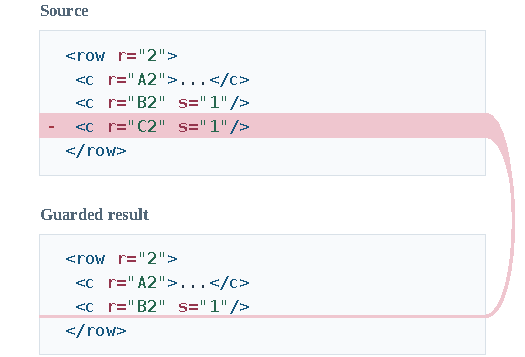
\includegraphics[width=\columnwidth]{figures/xml-methods/font-witness-code.pdf}
\par\smallskip
\begin{tabular}{@{}l@{\hspace{0.02\columnwidth}}c@{}}
Original & 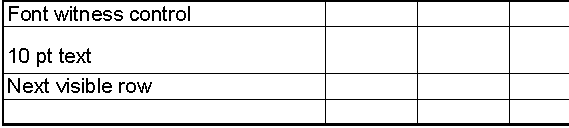
\includegraphics[width=0.70\columnwidth]{evidence/xml-methods/native-vector/font/source.pdf} \\
One witness & 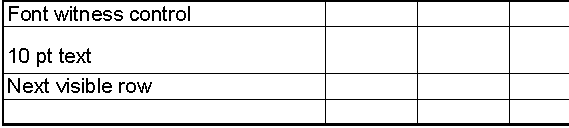
\includegraphics[width=0.70\columnwidth]{evidence/xml-methods/native-vector/font/one-witness.pdf} \\
No witness & 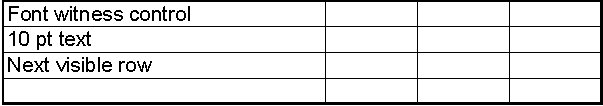
\includegraphics[width=0.70\columnwidth]{evidence/xml-methods/native-vector/font/no-witness.pdf}
\end{tabular}
\caption{Font-witness control. A2 uses Arial 10; empty B2 and C2 use Arial 18.
Retaining either blank preserves the rebuilt rendering. Removing both reduces
row 2 from 23.25 to 12.75 points and shifts the following row. XML is abbreviated;
images are native Excel print exports.}
\label{fig:font-witness-native}
\end{figure}
